\chapter{ӨГӨГДӨЛ ЦУГЛУУЛАЛТ БА БОЛОВСРУУЛАЛТ}
\section{Монгол улсын дугаарын бүтэц}
Монгол улсын хувийн тээврийн хэрэгслийн дугаар нь дөрвөн орон (тэргүүн тэг зөвшөөрнө) ба гурван том кирилл үсгээс бүрдэнэ, жишээ нь \plate{1234 УБА}~\cite{wikimn}. Эхний хоёр үсэг нь бүртгэсэн аймаг эсвэл хотын код (УБ, УН, УА, УЕ, УК --- Улаанбаатар; АР --- Архангай; ДА --- Дархан-Уул; ОР --- Орхон; СЭ --- Сэлэнгэ; ТӨ --- Төв гэх мэт, бүрэн жагсаалт Хавсралт~\ref{app:regions}), гурав дахь үсэг нь серийн үсэг. 2001 оноос дугаарын зүүн талд улаан Соёмбо, тоо ба үсгийн хооронд ``MNG'' зууван тэмдэг нэмэгдсэн; фонт нь DIN 1451 байсан бол 2018 оноос Roboto болсон. Хуучин дугаарт тооны хоёр хосын хооронд зураас байдаг (\plate{91-44 УБА}). Дугаар нэг мөрт (520$\times$110~мм) ба хоёр мөрт дөрвөлжин (дээд мөрөнд тоо, доод мөрөнд үсэг) гэсэн хоёр физик хэлбэртэй. Дипломат дугаар улаан өнгөтэй, ДК-ээр эхэлдэг; цэргийн (ЦАБ), хилийн (ХЦА) тусгай цуврал байдаг~\cite{dierkes2019}. Зураг~\ref{fig:samples}-д бодит жишээг үзүүлэв.
\begin{figure}[H]\centering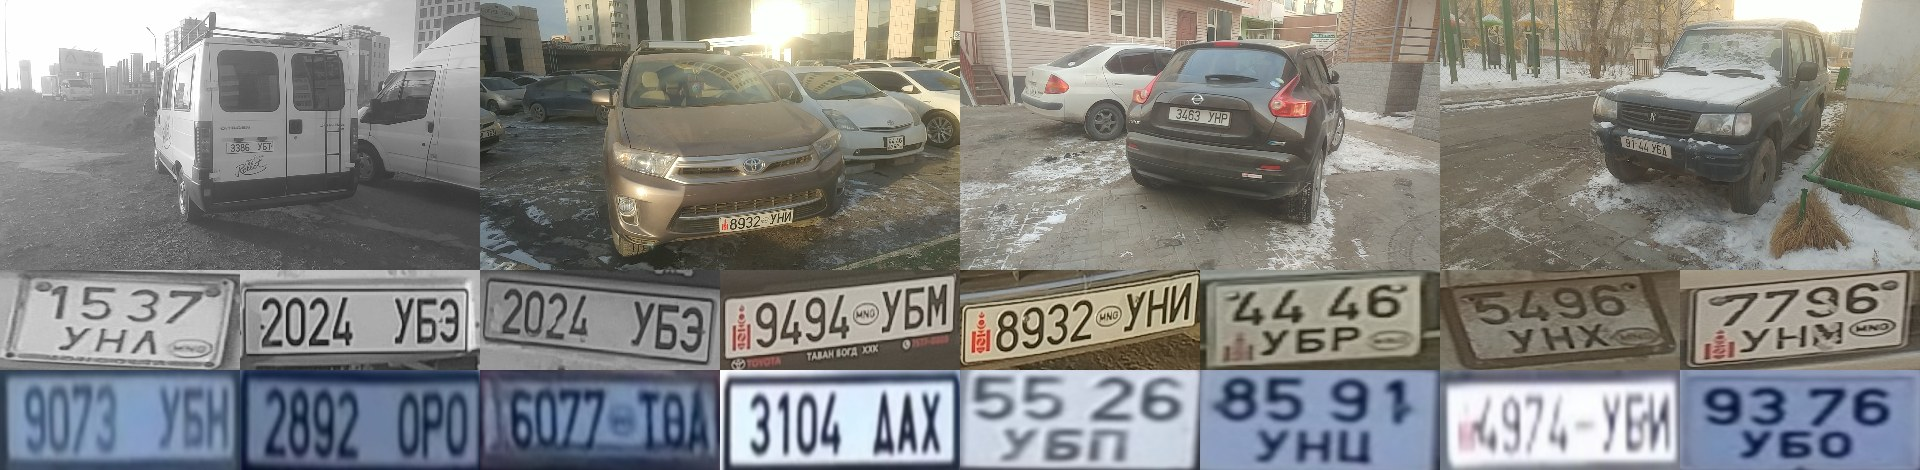
\includegraphics[width=\textwidth]{samples_real.jpg}
\caption{Бодит өгөгдлийн жишээ. Дээд мөр: gumbernator/Mongolian-ALPR олонлогийн бүтэн дүрстэй зураг (Улаанбаатар, зогсоол, өвлийн өдөр, гар утас, 1920$\times$1080). Дунд мөр: тэдгээрийн дугаарын тайралт --- нэг мөрт, зураастай хуучин, хоёр мөрт хэлбэрүүд. Доод мөр: MLUB тэмцээний замын камерын тайралт (470$\times$110, хоёр мөрт дугаар сунгагдсан).}\label{fig:samples}\end{figure}

\section{Өгөгдлийн эх үүсвэрүүд}
Нээлттэй эх үүсвэрийг GitHub, Roboflow Universe, HuggingFace, Kaggle дээр хайж, олдсон бүх зүйлийг Хүснэгт~\ref{tab:sources}-д нэгтгэв. Хэмжээг Зураг~\ref{fig:dataset}-д харуулав.
\begin{table}[H]\centering\caption{Судалсан өгөгдлийн эх үүсвэрүүд ба тэдгээрийн ашиглалт}\label{tab:sources}\footnotesize
\begin{tabular}{p{4.2cm}p{2.2cm}p{3cm}p{5.2cm}}\toprule
Эх үүсвэр & Хэмжээ & Шошго & Ашиглалт\\\midrule
gumbernator/Mongolian-ALPR (GitHub, Apache-2.0)~\cite{gumbernator} & 68 зураг 1920$\times$1080, 74 дугаар & Pascal VOC: дугаарын хайрцаг + тэмдэгт бүрийн хайрцаг (латин галиг) & тэмдэгтийн хайрцгаас 72 дугаарын текст сэргээсэн; илрүүлэгчийн тохируулга (48), уншигчийн тохируулга (74 мөр), төгсгөл хүртэлх тест (18 зураг, 19 дугаар)\\
MLUB ``Mongolian car plate prediction'' (Tsundgerhen репо дотор)~\cite{tsund} & 7\,394 тайралт 470$\times$110, 5\,575 ялгаатай дугаар & \texttt{training.csv}, \texttt{test.csv}: дугаарын текст & дүрэмд нийцэхгүй 2-ыг хасч 7\,392; уншигчийн гол сургалт (5\,901) ба тест (1\,491)\\
keremberke/license-plate-object-detection (HuggingFace) & 8\,823 зураг (6\,176/1\,765/882) & COCO хайрцаг, 1 анги & илрүүлэгчийн урьдчилсан сургалт (A үе), тест\\
Roboflow Universe computer-vision-m1xzb/mongolian-plate~\cite{roboflowmn} & 984 зураг, 2 хувилбар (2025-04-13) & зөвхөн хайрцаг, CC BY 4.0 & татахад бүртгэл, API түлхүүр шаардлагатай тул татаагүй; \texttt{scripts/download\_roboflow.py} бэлэн\\
Синтетик үүсгэгч (энэ ажил) & 60\,000 дугаар $\to$ 90\,021 мөр & текст & уншигчийн урьдчилсан сургалт\\
Tsundgerhen репогийн бичлэг & 3 бичлэг, 30 fps & шошгогүй & олон кадрын чанарын туршилт\\
Kaggle mlub-mongolian-car-plate-prediction-v1 & 34 KB CSV & текст, зураггүй & ашиглаагүй\\\bottomrule
\end{tabular}\end{table}
\begin{figure}[H]\centering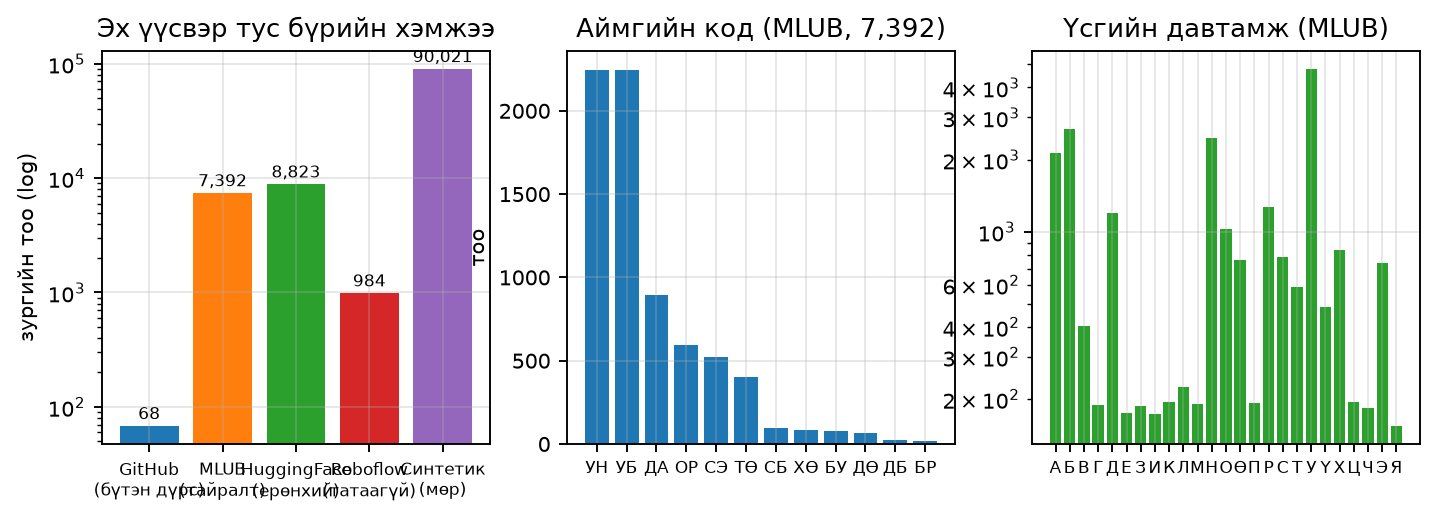
\includegraphics[width=\textwidth]{dataset_overview.png}
\caption{Өгөгдлийн тойм: эх үүсвэр тус бүрийн хэмжээ (зүүн, логарифм), MLUB дугаарын аймгийн кодын тархалт (дунд), MLUB дугаарын үсгийн давтамж (баруун, логарифм). Аймгийн кодоос болж У, Б, Н, А үсэг давамгайлж, серийн үсгүүд ховор байна.}\label{fig:dataset}\end{figure}

\section{Тэмдэгтийн хайрцгаас текст сэргээх}
gumbernator олонлогийн XML файлд дугаарын хайрцаг ба тэмдэгт бүрийн хайрцаг латин галигаар (\texttt{uu}=Ү, \texttt{q}=Ө, \texttt{ye}=Е, \texttt{e}=Э, \texttt{ts}=Ц, \texttt{ch}=Ч, \texttt{ya}=Я гэх мэт) шошголсон байв. Галигийг тэмдэгт бүрийн тайралтыг нүдээр шалгаж баталгаажуулсан. Дугаар тус бүрт түүний дотор орших тэмдэгтийн хайрцгуудыг тоо ба үсэг гэж салгаж, $x$ координатаар эрэмбэлж залгахад дугаарын текст гарна; 4 орон + 3 үсэг бүрдээгүй 2 дугаарыг хаяж 72 дугаар авав. Хоёр мөрт дугаарын хувьд тооны хайрцгуудын нэгдэл ба үсгийн хайрцгуудын нэгдлийг тус тусад нь мөрийн тайралт болгож (\plate{1537} ба \plate{УНЛ}), нэг мөрт дугаарыг бүтнээр нь нэг мөр болгов. Дугаарын хайрцгийн өргөн/өндрийн харьцаа хоёр хэлбэрийг цэвэр ялгаж байгааг Зураг~\ref{fig:aspect}-д харуулав: хоёр мөрт 0.98--1.53, нэг мөрт 1.89--3.81, босго 1.8.
\begin{figure}[H]\centering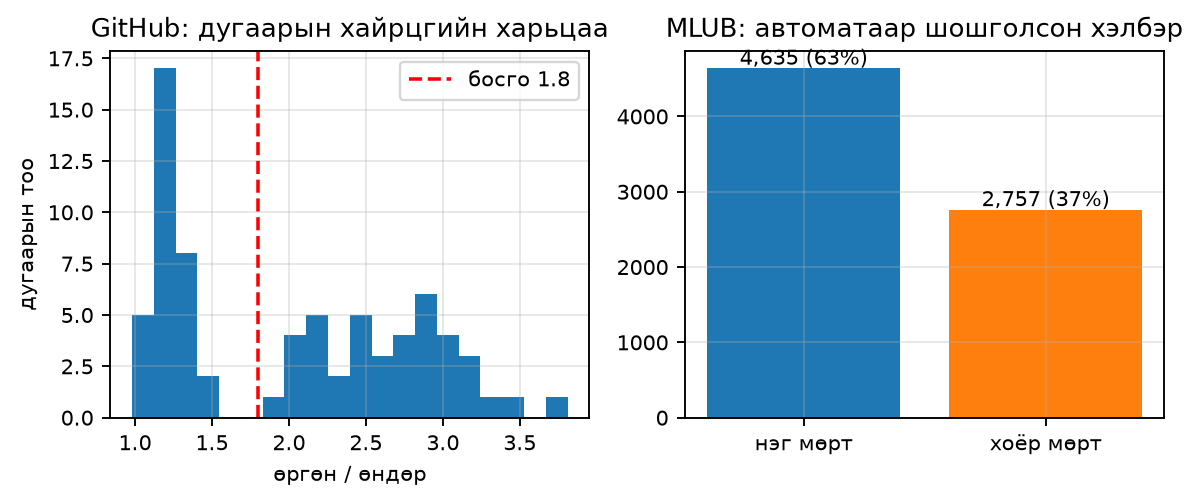
\includegraphics[width=0.95\textwidth]{aspect_layout.png}
\caption{Зүүн: GitHub олонлогийн дугаарын хайрцгийн өргөн/өндөр харьцааны гистограм ба 1.8 босго. Баруун: MLUB тайралтын автоматаар шошголсон хэлбэр (2\,757 буюу 37 хувь нь хоёр мөрт).}\label{fig:aspect}\end{figure}

\section{MLUB тайралтын хэлбэрийг автоматаар шошголох}
MLUB-ийн бүх зураг 470$\times$110 болгож сунгасан тул хоёр мөрт дугаарын хэлбэрийг харьцаагаар ялгах боломжгүй, хэлбэрийн шошго ч байхгүй. Уншигч нэг мөрийг л уншдаг тул сургалтын өмнө хэлбэрийг тодорхойлох шаардлагатай. Үүнд одоо байгаа уншигчийг ашиглан дараах дүрмийг хэрэглэв: (а) зургийг бүтнээр нь уншина; (б) дээд 55 хувь ба доод 55 хувийг тусад нь уншиж залгана; (б) үнэн текстийг яг гаргавал хоёр мөрт, үгүй бол (а) гаргавал нэг мөрт; аль нь ч биш бол засварлах зайгаар (edit distance) ойр нь; тэнцвэл хэвтээ бэхний профилийн тест. Хоёр хагасыг тусад нь уншихад тоо ба үсэг яг гарах нь зөвхөн хоёр мөртэй зурагт боломжтой тул хуваасан тестийг давуу эрхтэй болгосон. Анхны хувилбарт зайн зөрүүг 2-оос багагүй шаардсан нь хоёр мөртийг 571 гэж дутуу шошголсон; дүрмийг засч дахин ажиллуулахад 2\,757 хоёр мөрт (37 хувь), тэнцсэн 87 тохиолдол гарсан. Нэг мөрт гэж шошголсон 36 санамсаргүй зургийг нүдээр шалгахад 1 нь хоёр мөрт байсан тул шошгоны алдаа 3 хувь орчим гэж үзэв.

\section{Сургалт, шалгалтын хуваалт}
Бүх хуваалтыг \emph{дугаарын текстээр} хийв: нэг машин хэд хэдэн зурагт байвал бүгд нэг талд орно (Зураг~\ref{fig:splits}). GitHub олонлогийг 70/30 хуваахад 48 сургалт / 18 шалгалтын зураг (53 / 19 дугаар, 74 / 30 мөр), давхцал тэг. MLUB-ийн тэмцээний анхны training/test хуваалтыг ашиглах боломжгүй, учир нь тестийн зураг нь сургалтын машинуудын нэмэлт кадрууд (3\,150 дугаар давхцсан); иймд 5\,575 ялгаатай дугаарыг 80/20 хуваахад 5\,901 сургалт / 1\,491 тестийн тайралт (8\,094 / 2\,055 мөр), давхцал тэг. HuggingFace олонлогийн анхны 6\,176/1\,765/882 хуваалтыг хэвээр ашиглав. GitHub олонлог нь камер, зургийн хүрээ (бүтэн машин, гар утас) өөр тул илрүүлэгч + уншигчийн төгсгөл хүртэлх тестийн үүрэг гүйцэтгэнэ.
\begin{figure}[H]\centering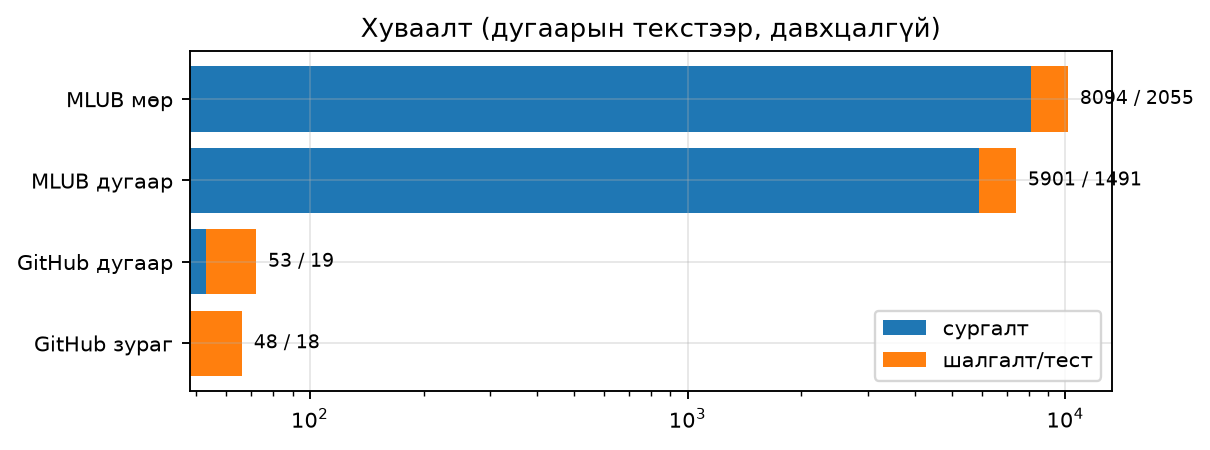
\includegraphics[width=0.85\textwidth]{splits.png}
\caption{Хуваалтын хэмжээ (логарифм тэнхлэг). Бүх хуваалт дугаарын текстээр хийгдсэн тул нэг дугаар сургалт, шалгалтын аль алинд байхгүй.}\label{fig:splits}\end{figure}

\section{Синтетик дугаар үүсгэх}
Уншигч 45 тэмдэгтийн ангийг 74 бодит мөрөөс сурах боломжгүй тул монгол дугаарын дизайныг дуурайсан синтетик үүсгэгч бичив (\texttt{scripts/synth\_plates.py}, Зураг~\ref{fig:synth}). Нэг дээж үүсэх алхмууд:
\begin{enumerate}[leftmargin=2.5em]
\item \textbf{Текст.} Дөрвөн орон санамсаргүй; аймгийн код 29 кодоос ажиглагдсан давтамжаар жинлэж (УБ 40, УН 25, УА 6, УЕ 4, УК 3 хувь, бусад тус бүр 1.2 хувь орчим), 10 хувьд бүрэн санамсаргүй хоёр үсэг (35 үсэг бүгд сургалтад орох үүднээс); серийн үсэг дугаар дээр ажиглагдсан 25 үсгээс 90 хувь, бүх үсгээс 10 хувь.
\item \textbf{Зурах.} PIL сангаар цагаан дэвсгэр (RGB 225--255), хар хүрээ (3--10~px), бэх (0--30). Нэг мөрт 1040$\times$220~px (50 хувь): Соёмбо + тоо + MNG зууван + үсэг (55 хувь), зураастай хуучин хэлбэр (25 хувь), энгийн (20 хувь). Хоёр мөрт 300--360$\times$220--280~px (50 хувь): дээд мөр Соёмбо + тоо, доод мөр үсэг; үүнээс дээд ба доод мөрийн хоёр тайралт гаргана. Соёмбог яг хуулбарлах фонт байхгүй тул улаан гал, нар, сар, зураасны баганаар ойролцоо зурсан. Есөн кирилл фонт (Roboto, Roboto Flex, Roboto Mono, PT Sans Bold, Fira Sans Condensed Medium/SemiBold, Oswald, DejaVu Sans Bold/Condensed Bold, Noto Sans Condensed/SemiCondensed Bold); хувьсах фонтод жин $\{500,600,700\}$, өргөн $\{75,87,100\}$ санамсаргүй.
\item \textbf{Аугментаци} (Хүснэгт~\ref{tab:aug}): илрүүлэгчийн хайрцгийн алдааг дуурайсан захын шилжилт, перспектив, эргүүлэлт, нягтрал бууруулалт, гэрлийн өөрчлөлт, сүүдэр, шороо, шуугиан, бүдэг, JPEG шахалт.
\end{enumerate}
60\,000 дугаараас 90\,021 мөр зураг (нэг мөрт 1, хоёр мөрт 2 мөр) үүсгэхэд 5 минут зарцуулав.
\begin{table}[H]\centering\caption{Синтетик дугаарын аугментацийн параметрүүд}\label{tab:aug}\small
\begin{tabular}{llc}\toprule
Хувиргалт & Параметр & Магадлал\\\midrule
Захын шилжилт (тайралтын зах) & өндөр/өргөний $-4\ldots+12$ хувь, дурын өнгөт зах & 1.0\\
Перспектив & булан $\pm8$ хувь өргөн, $\pm12$ хувь өндөр & 0.8\\
Эргүүлэлт & $\pm8^\circ$ & 0.7\\
Нягтрал бууруулах & өндөр $\{14,16,20,24,24,28,32,32,40,48,64\}$~px & 1.0\\
Тод байдал, offset & $\times0.55\ldots1.25$, $\pm35$ & 1.0\\
Өнгөний хазайлт & суваг бүрт $\pm15$ & 1.0\\
Гамма & $0.6\ldots1.6$ & 0.5\\
Сүүдрийн зурвас & санамсаргүй дөрвөлжин, 50 хувь харанхуй & 0.4\\
Шороо, толбо & 1--5 тойрог, радиус 1--4 & 0.3\\
Gaussian шуугиан & $\sigma\in[0,12]$ & 1.0\\
Gaussian бүдэг & цөм 3 эсвэл 5 & 0.5\\
Хөдөлгөөний бүдэг & цөм 3, 5, 7 (хэвтээ) & 0.3\\
JPEG дахин шахалт & чанар 30--90 & 0.6\\
Хар цагаан & & 0.15\\\bottomrule
\end{tabular}\end{table}
\begin{figure}[H]\centering
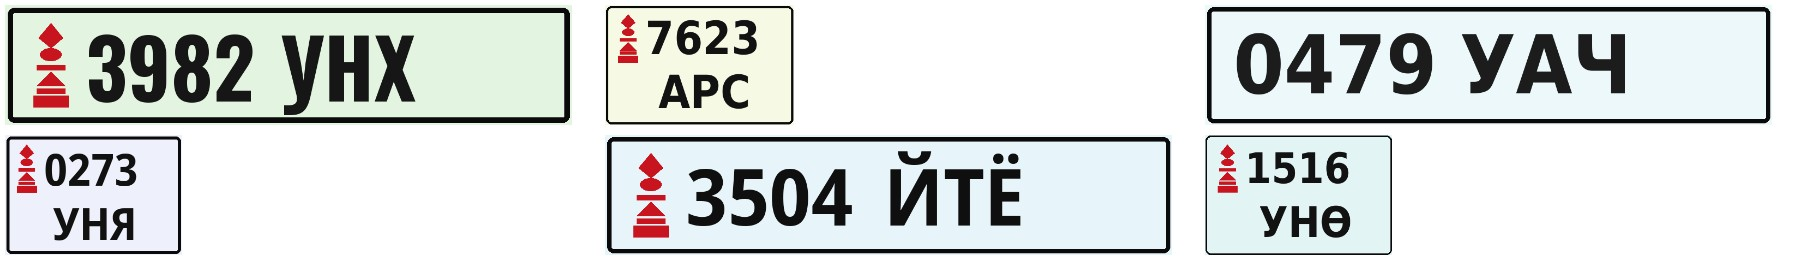
\includegraphics[width=\textwidth]{samples_synth_clean.jpg}\\[2pt]
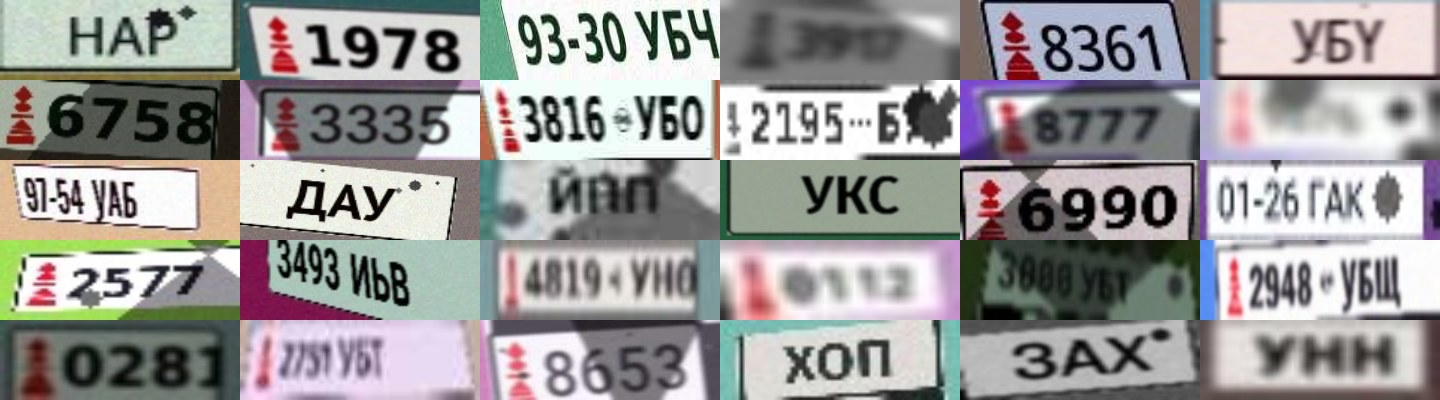
\includegraphics[width=\textwidth]{samples_synth.jpg}
\caption{Синтетик дугаар. Дээд: аугментацийн өмнөх цэвэр рендер (нэг ба хоёр мөрт, Соёмбо, MNG зууван, өөр фонтууд). Доод: аугментацийн дараах сургалтын мөр зургууд (нэг мөрт бүтэн дугаар, хоёр мөрт дугаарын тооны мөр ба үсгийн мөр).}\label{fig:synth}\end{figure}

\section{Шошгоны чанар ба хязгаарлалт}
GitHub олонлогийн тэмдэгтийн шошгыг нүдээр шалгахад галигийн андуурал олдоогүй; тэмдэгт дутуу 2 дугаарыг хассан. MLUB-ийн текст нь тэмцээний зохион байгуулагчийн шошго бөгөөд дүрэмд нийцэхгүй 2 бичлэг (\plate{80213МР}, \plate{0999ТЧ}) олдсон нь шошгоны чанар өндөр гэдгийг илтгэнэ; харин хэлбэрийн шошго автомат тул 3 хувь орчим алдаатай, энэ нь сургалтад хэдэн буруу мөр оруулж, тестэд алдаа гэж тоологдоно. Бодит зураг бүгд өдрийн гэрэлд авсан; шөнө, бороо, гэрлийн гялбааг зөвхөн аугментаци дуурайж байгаа нь энэ өгөгдлийн гол хязгаарлалт юм.
